\documentclass[a4paper,17pt]{extarticle}


    \usepackage[sfdefault, condensed]{roboto} % police d'écriture plus moderne
\usepackage[french]{babel} % francisation
\usepackage[parfill]{parskip} %suppression indentation

\usepackage{fancyhdr}
\usepackage{multicol}

% figure non flotantes
\usepackage{float}
\let\origfigure\figure
\let\endorigfigure\endfigure
\renewenvironment{figure}[1][2] {
    \expandafter\origfigure\expandafter[H]
} {
    \endorigfigure
}

% mois/année
\usepackage{datetime}
\newdateformat{monthyeardate}{%
  \monthname[\THEMONTH] \THEYEAR}

% couleurs perso
\usepackage[table]{xcolor}
\definecolor{deepblue}{rgb}{0.3,0.3,0.8}
\definecolor{darkblue}{rgb}{0,0,0.3}
\definecolor{deepred}{rgb}{0.6,0,0}
\definecolor{iremred}{RGB}{204,35,50}
\definecolor{deepgreen}{rgb}{0,0.6,0}
\definecolor{backcolor}{rgb}{0.98,0.95,0.95}
\definecolor{grisClair}{rgb}{0.95,0.95,0.95}
\definecolor{orangeamu}{RGB}{250,178,11}
\definecolor{noiramu}{RGB}{35,31,32}
\definecolor{bleuamu}{RGB}{20,118,198}
\definecolor{bleuamudark}{RGB}{15,90,150}
\definecolor{cyanamu}{RGB}{77,198,244}


\usepackage{/home/bouscadilla/Documents/Code/nbconvert/template/latex/pdf_solution/xeboiboites}
%
% exemple
\newbreakabletheorem[
    small box style={fill=deepblue!90,draw=deepblue!15, rounded corners,line width=1pt},%
    big box style={fill=deepblue!5,draw=deepblue!15,thick,rounded corners,line width=1pt},%
    headfont={\color{white}\bfseries}
        ]{exemple}{Exemple}{}%{counterCo}
%
% remarque
\newbreakabletheorem[
    small box style={draw=ansi-green-intense!100,line width=2pt,fill=ansi-green-intense!0,rounded corners,decoration=penciline, decorate},%
	big box style={color=ansi-green-intense!90,fill=ansi-green-intense!10,thick,decoration={penciline},decorate},
    broken edges={draw=ansi-green-intense!90,thick,fill=orange!20!black!5, decoration={random steps, segment length=.5cm,amplitude=1.3mm},decorate},%
    other edges={decoration=penciline,decorate,thick},%
    headfont={\color{ansi-green-intense}\large\scshape\bfseries}
    ]{remarque}{Remarque}{}%{counterCa}
%
% formule (sans titre)
\newboxedequation[%
    big box style={fill=cyanamu!10,draw=cyanamu!100,thick,decoration=penciline,decorate}]%
    {form}
%
% Réponse
\newbreakabletheorem[
    small box style={fill=bleuamu!100, draw=bleuamu!60, line width=1pt,rounded corners,decorate},%
    big box style={fill=bleuamu!10,draw=bleuamu!30,thick,rounded corners,decorate},
    headfont={\color{white}\large\scshape\bfseries}
        ]{reponse}{Correction}{}
%

%
% À retenir
%\newbreakabletheorem[
%    small box style={fill=deepred!100, draw=deepred!80, line width=1pt,rounded corners,decorate},%
%    big box style={fill=deepred!10,draw=deepred!50,thick,rounded corners,decorate},
%    headfont={\color{white}\large\scshape\bfseries}
%        ]{retenir}{À retenir}{}
%
\newboxedequation[%
    big box style={fill=deepred!10,draw=deepred!0,thick,decoration=penciline,decorate}]%
    {retenir}



% astuce
\newspanning[
    image=/home/bouscadilla/Documents/Code/nbconvert/template/latex/pdf_solution/fig-idee,headfont=\bfseries,
    spanning style={very thick,decoration=penciline,decorate}
    ]{astuce}{Astuce}{}
%
% activité

\newcounter{counterCa}
\newbreakabletheorem[
    small box style={draw=orangeamu!100,line width=2pt,fill=orangeamu!100,rounded corners,decoration=penciline, decorate},%
	big box style={color=orangeamu!100,fill=orangeamu!5,thick,decoration={penciline},decorate},
    broken edges={draw=orangeamu!100,thick,fill=orangeamu!100, decoration={random steps, segment length=.5cm,amplitude=1.3mm},decorate},%
    other edges={decoration=penciline,decorate,thick},%
    headfont={\color{white}\large\scshape\bfseries}
    ]{activite}{\adjustimage{height=1cm, valign=m}{/home/bouscadilla/Documents/Code/nbconvert/template/latex/pdf_solution/papier_eleve_investigation.png}%
    Activité}{counterCa}
%   
%   environnement élève
%
\newenvironment{eleve}%
%{\begin{activite}\large\\} % écrire plus gros
{\begin{activite}\color{noiramu}\\[-0.5cm]}
{\end{activite}}

\newenvironment{formule}%
%{\begin{activite}\large\\} % écrire plus gros
{\begin{form}\color{bleuamu}}
{\end{form}}


\usepackage[breakable]{tcolorbox}
    \usepackage{parskip} % Stop auto-indenting (to mimic markdown behaviour)
    
    \usepackage{iftex}
    \ifPDFTeX
    	\usepackage[T1]{fontenc}
    	\usepackage{mathpazo}
    \else
    	\usepackage{fontspec}
    \fi

    % Basic figure setup, for now with no caption control since it's done
    % automatically by Pandoc (which extracts ![](path) syntax from Markdown).
    \usepackage{graphicx}
    % Maintain compatibility with old templates. Remove in nbconvert 6.0
    \let\Oldincludegraphics\includegraphics
    % Ensure that by default, figures have no caption (until we provide a
    % proper Figure object with a Caption API and a way to capture that
    % in the conversion process - todo).
    \usepackage{caption}
    \DeclareCaptionFormat{nocaption}{}
    \captionsetup{format=nocaption,aboveskip=0pt,belowskip=0pt}

    \usepackage[Export]{adjustbox} % Used to constrain images to a maximum size
    \adjustboxset{max size={0.9\linewidth}{0.9\paperheight}}
    \usepackage{float}
    \floatplacement{figure}{H} % forces figures to be placed at the correct location
    \usepackage{xcolor} % Allow colors to be defined
    \usepackage{enumerate} % Needed for markdown enumerations to work
    \usepackage{geometry} % Used to adjust the document margins
    \usepackage{amsmath} % Equations
    \usepackage{amssymb} % Equations
    \usepackage{textcomp} % defines textquotesingle
    % Hack from http://tex.stackexchange.com/a/47451/13684:
    \AtBeginDocument{%
        \def\PYZsq{\textquotesingle}% Upright quotes in Pygmentized code
    }
    \usepackage{upquote} % Upright quotes for verbatim code
    \usepackage{eurosym} % defines \euro
    \usepackage[mathletters]{ucs} % Extended unicode (utf-8) support
    \usepackage{fancyvrb} % verbatim replacement that allows latex

    % The hyperref package gives us a pdf with properly built
    % internal navigation ('pdf bookmarks' for the table of contents,
    % internal cross-reference links, web links for URLs, etc.)
    \usepackage{hyperref}
    % The default LaTeX title has an obnoxious amount of whitespace. By default,
    % titling removes some of it. It also provides customization options.
    \usepackage{titling}
    \usepackage{longtable} % longtable support required by pandoc >1.10
    \usepackage{booktabs}  % table support for pandoc > 1.12.2
    \usepackage[inline]{enumitem} % IRkernel/repr support (it uses the enumerate* environment)
    \usepackage[normalem]{ulem} % ulem is needed to support strikethroughs (\sout)
                                % normalem makes italics be italics, not underlines
    \usepackage{mathrsfs}
    

    
    % Colors for the hyperref package
    \definecolor{urlcolor}{rgb}{0,.145,.698}
    \definecolor{linkcolor}{rgb}{.71,0.21,0.01}
    \definecolor{citecolor}{rgb}{.12,.54,.11}

    % ANSI colors
    \definecolor{ansi-black}{HTML}{3E424D}
    \definecolor{ansi-black-intense}{HTML}{282C36}
    \definecolor{ansi-red}{HTML}{E75C58}
    \definecolor{ansi-red-intense}{HTML}{B22B31}
    \definecolor{ansi-green}{HTML}{00A250}
    \definecolor{ansi-green-intense}{HTML}{007427}
    \definecolor{ansi-yellow}{HTML}{DDB62B}
    \definecolor{ansi-yellow-intense}{HTML}{B27D12}
    \definecolor{ansi-blue}{HTML}{208FFB}
    \definecolor{ansi-blue-intense}{HTML}{0065CA}
    \definecolor{ansi-magenta}{HTML}{D160C4}
    \definecolor{ansi-magenta-intense}{HTML}{A03196}
    \definecolor{ansi-cyan}{HTML}{60C6C8}
    \definecolor{ansi-cyan-intense}{HTML}{258F8F}
    \definecolor{ansi-white}{HTML}{C5C1B4}
    \definecolor{ansi-white-intense}{HTML}{A1A6B2}
    \definecolor{ansi-default-inverse-fg}{HTML}{FFFFFF}
    \definecolor{ansi-default-inverse-bg}{HTML}{000000}

    % commands and environments needed by pandoc snippets
    % extracted from the output of `pandoc -s`
    \providecommand{\tightlist}{%
      \setlength{\itemsep}{0pt}\setlength{\parskip}{0pt}}
    \DefineVerbatimEnvironment{Highlighting}{Verbatim}{commandchars=\\\{\}}
    % Add ',fontsize=\small' for more characters per line
    \newenvironment{Shaded}{}{}
    \newcommand{\KeywordTok}[1]{\textcolor[rgb]{0.00,0.44,0.13}{\textbf{{#1}}}}
    \newcommand{\DataTypeTok}[1]{\textcolor[rgb]{0.56,0.13,0.00}{{#1}}}
    \newcommand{\DecValTok}[1]{\textcolor[rgb]{0.25,0.63,0.44}{{#1}}}
    \newcommand{\BaseNTok}[1]{\textcolor[rgb]{0.25,0.63,0.44}{{#1}}}
    \newcommand{\FloatTok}[1]{\textcolor[rgb]{0.25,0.63,0.44}{{#1}}}
    \newcommand{\CharTok}[1]{\textcolor[rgb]{0.25,0.44,0.63}{{#1}}}
    \newcommand{\StringTok}[1]{\textcolor[rgb]{0.25,0.44,0.63}{{#1}}}
    \newcommand{\CommentTok}[1]{\textcolor[rgb]{0.38,0.63,0.69}{\textit{{#1}}}}
    \newcommand{\OtherTok}[1]{\textcolor[rgb]{0.00,0.44,0.13}{{#1}}}
    \newcommand{\AlertTok}[1]{\textcolor[rgb]{1.00,0.00,0.00}{\textbf{{#1}}}}
    \newcommand{\FunctionTok}[1]{\textcolor[rgb]{0.02,0.16,0.49}{{#1}}}
    \newcommand{\RegionMarkerTok}[1]{{#1}}
    \newcommand{\ErrorTok}[1]{\textcolor[rgb]{1.00,0.00,0.00}{\textbf{{#1}}}}
    \newcommand{\NormalTok}[1]{{#1}}
    
    % Additional commands for more recent versions of Pandoc
    \newcommand{\ConstantTok}[1]{\textcolor[rgb]{0.53,0.00,0.00}{{#1}}}
    \newcommand{\SpecialCharTok}[1]{\textcolor[rgb]{0.25,0.44,0.63}{{#1}}}
    \newcommand{\VerbatimStringTok}[1]{\textcolor[rgb]{0.25,0.44,0.63}{{#1}}}
    \newcommand{\SpecialStringTok}[1]{\textcolor[rgb]{0.73,0.40,0.53}{{#1}}}
    \newcommand{\ImportTok}[1]{{#1}}
    \newcommand{\DocumentationTok}[1]{\textcolor[rgb]{0.73,0.13,0.13}{\textit{{#1}}}}
    \newcommand{\AnnotationTok}[1]{\textcolor[rgb]{0.38,0.63,0.69}{\textbf{\textit{{#1}}}}}
    \newcommand{\CommentVarTok}[1]{\textcolor[rgb]{0.38,0.63,0.69}{\textbf{\textit{{#1}}}}}
    \newcommand{\VariableTok}[1]{\textcolor[rgb]{0.10,0.09,0.49}{{#1}}}
    \newcommand{\ControlFlowTok}[1]{\textcolor[rgb]{0.00,0.44,0.13}{\textbf{{#1}}}}
    \newcommand{\OperatorTok}[1]{\textcolor[rgb]{0.40,0.40,0.40}{{#1}}}
    \newcommand{\BuiltInTok}[1]{{#1}}
    \newcommand{\ExtensionTok}[1]{{#1}}
    \newcommand{\PreprocessorTok}[1]{\textcolor[rgb]{0.74,0.48,0.00}{{#1}}}
    \newcommand{\AttributeTok}[1]{\textcolor[rgb]{0.49,0.56,0.16}{{#1}}}
    \newcommand{\InformationTok}[1]{\textcolor[rgb]{0.38,0.63,0.69}{\textbf{\textit{{#1}}}}}
    \newcommand{\WarningTok}[1]{\textcolor[rgb]{0.38,0.63,0.69}{\textbf{\textit{{#1}}}}}
    
    
    % Define a nice break command that doesn't care if a line doesn't already
    % exist.
    \def\br{\hspace*{\fill} \\* }
    % Math Jax compatibility definitions
    \def\gt{>}
    \def\lt{<}
    \let\Oldtex\TeX
    \let\Oldlatex\LaTeX
    \renewcommand{\TeX}{\textrm{\Oldtex}}
    \renewcommand{\LaTeX}{\textrm{\Oldlatex}}
    % Document parameters
    % Document title
    \title{2-3---bases-python-microbit}
    
    
    
    
    
% Pygments definitions
\makeatletter
\def\PY@reset{\let\PY@it=\relax \let\PY@bf=\relax%
    \let\PY@ul=\relax \let\PY@tc=\relax%
    \let\PY@bc=\relax \let\PY@ff=\relax}
\def\PY@tok#1{\csname PY@tok@#1\endcsname}
\def\PY@toks#1+{\ifx\relax#1\empty\else%
    \PY@tok{#1}\expandafter\PY@toks\fi}
\def\PY@do#1{\PY@bc{\PY@tc{\PY@ul{%
    \PY@it{\PY@bf{\PY@ff{#1}}}}}}}
\def\PY#1#2{\PY@reset\PY@toks#1+\relax+\PY@do{#2}}

\expandafter\def\csname PY@tok@w\endcsname{\def\PY@tc##1{\textcolor[rgb]{0.73,0.73,0.73}{##1}}}
\expandafter\def\csname PY@tok@c\endcsname{\let\PY@it=\textit\def\PY@tc##1{\textcolor[rgb]{0.25,0.50,0.50}{##1}}}
\expandafter\def\csname PY@tok@cp\endcsname{\def\PY@tc##1{\textcolor[rgb]{0.74,0.48,0.00}{##1}}}
\expandafter\def\csname PY@tok@k\endcsname{\let\PY@bf=\textbf\def\PY@tc##1{\textcolor[rgb]{0.00,0.50,0.00}{##1}}}
\expandafter\def\csname PY@tok@kp\endcsname{\def\PY@tc##1{\textcolor[rgb]{0.00,0.50,0.00}{##1}}}
\expandafter\def\csname PY@tok@kt\endcsname{\def\PY@tc##1{\textcolor[rgb]{0.69,0.00,0.25}{##1}}}
\expandafter\def\csname PY@tok@o\endcsname{\def\PY@tc##1{\textcolor[rgb]{0.40,0.40,0.40}{##1}}}
\expandafter\def\csname PY@tok@ow\endcsname{\let\PY@bf=\textbf\def\PY@tc##1{\textcolor[rgb]{0.67,0.13,1.00}{##1}}}
\expandafter\def\csname PY@tok@nb\endcsname{\def\PY@tc##1{\textcolor[rgb]{0.00,0.50,0.00}{##1}}}
\expandafter\def\csname PY@tok@nf\endcsname{\def\PY@tc##1{\textcolor[rgb]{0.00,0.00,1.00}{##1}}}
\expandafter\def\csname PY@tok@nc\endcsname{\let\PY@bf=\textbf\def\PY@tc##1{\textcolor[rgb]{0.00,0.00,1.00}{##1}}}
\expandafter\def\csname PY@tok@nn\endcsname{\let\PY@bf=\textbf\def\PY@tc##1{\textcolor[rgb]{0.00,0.00,1.00}{##1}}}
\expandafter\def\csname PY@tok@ne\endcsname{\let\PY@bf=\textbf\def\PY@tc##1{\textcolor[rgb]{0.82,0.25,0.23}{##1}}}
\expandafter\def\csname PY@tok@nv\endcsname{\def\PY@tc##1{\textcolor[rgb]{0.10,0.09,0.49}{##1}}}
\expandafter\def\csname PY@tok@no\endcsname{\def\PY@tc##1{\textcolor[rgb]{0.53,0.00,0.00}{##1}}}
\expandafter\def\csname PY@tok@nl\endcsname{\def\PY@tc##1{\textcolor[rgb]{0.63,0.63,0.00}{##1}}}
\expandafter\def\csname PY@tok@ni\endcsname{\let\PY@bf=\textbf\def\PY@tc##1{\textcolor[rgb]{0.60,0.60,0.60}{##1}}}
\expandafter\def\csname PY@tok@na\endcsname{\def\PY@tc##1{\textcolor[rgb]{0.49,0.56,0.16}{##1}}}
\expandafter\def\csname PY@tok@nt\endcsname{\let\PY@bf=\textbf\def\PY@tc##1{\textcolor[rgb]{0.00,0.50,0.00}{##1}}}
\expandafter\def\csname PY@tok@nd\endcsname{\def\PY@tc##1{\textcolor[rgb]{0.67,0.13,1.00}{##1}}}
\expandafter\def\csname PY@tok@s\endcsname{\def\PY@tc##1{\textcolor[rgb]{0.73,0.13,0.13}{##1}}}
\expandafter\def\csname PY@tok@sd\endcsname{\let\PY@it=\textit\def\PY@tc##1{\textcolor[rgb]{0.73,0.13,0.13}{##1}}}
\expandafter\def\csname PY@tok@si\endcsname{\let\PY@bf=\textbf\def\PY@tc##1{\textcolor[rgb]{0.73,0.40,0.53}{##1}}}
\expandafter\def\csname PY@tok@se\endcsname{\let\PY@bf=\textbf\def\PY@tc##1{\textcolor[rgb]{0.73,0.40,0.13}{##1}}}
\expandafter\def\csname PY@tok@sr\endcsname{\def\PY@tc##1{\textcolor[rgb]{0.73,0.40,0.53}{##1}}}
\expandafter\def\csname PY@tok@ss\endcsname{\def\PY@tc##1{\textcolor[rgb]{0.10,0.09,0.49}{##1}}}
\expandafter\def\csname PY@tok@sx\endcsname{\def\PY@tc##1{\textcolor[rgb]{0.00,0.50,0.00}{##1}}}
\expandafter\def\csname PY@tok@m\endcsname{\def\PY@tc##1{\textcolor[rgb]{0.40,0.40,0.40}{##1}}}
\expandafter\def\csname PY@tok@gh\endcsname{\let\PY@bf=\textbf\def\PY@tc##1{\textcolor[rgb]{0.00,0.00,0.50}{##1}}}
\expandafter\def\csname PY@tok@gu\endcsname{\let\PY@bf=\textbf\def\PY@tc##1{\textcolor[rgb]{0.50,0.00,0.50}{##1}}}
\expandafter\def\csname PY@tok@gd\endcsname{\def\PY@tc##1{\textcolor[rgb]{0.63,0.00,0.00}{##1}}}
\expandafter\def\csname PY@tok@gi\endcsname{\def\PY@tc##1{\textcolor[rgb]{0.00,0.63,0.00}{##1}}}
\expandafter\def\csname PY@tok@gr\endcsname{\def\PY@tc##1{\textcolor[rgb]{1.00,0.00,0.00}{##1}}}
\expandafter\def\csname PY@tok@ge\endcsname{\let\PY@it=\textit}
\expandafter\def\csname PY@tok@gs\endcsname{\let\PY@bf=\textbf}
\expandafter\def\csname PY@tok@gp\endcsname{\let\PY@bf=\textbf\def\PY@tc##1{\textcolor[rgb]{0.00,0.00,0.50}{##1}}}
\expandafter\def\csname PY@tok@go\endcsname{\def\PY@tc##1{\textcolor[rgb]{0.53,0.53,0.53}{##1}}}
\expandafter\def\csname PY@tok@gt\endcsname{\def\PY@tc##1{\textcolor[rgb]{0.00,0.27,0.87}{##1}}}
\expandafter\def\csname PY@tok@err\endcsname{\def\PY@bc##1{\setlength{\fboxsep}{0pt}\fcolorbox[rgb]{1.00,0.00,0.00}{1,1,1}{\strut ##1}}}
\expandafter\def\csname PY@tok@kc\endcsname{\let\PY@bf=\textbf\def\PY@tc##1{\textcolor[rgb]{0.00,0.50,0.00}{##1}}}
\expandafter\def\csname PY@tok@kd\endcsname{\let\PY@bf=\textbf\def\PY@tc##1{\textcolor[rgb]{0.00,0.50,0.00}{##1}}}
\expandafter\def\csname PY@tok@kn\endcsname{\let\PY@bf=\textbf\def\PY@tc##1{\textcolor[rgb]{0.00,0.50,0.00}{##1}}}
\expandafter\def\csname PY@tok@kr\endcsname{\let\PY@bf=\textbf\def\PY@tc##1{\textcolor[rgb]{0.00,0.50,0.00}{##1}}}
\expandafter\def\csname PY@tok@bp\endcsname{\def\PY@tc##1{\textcolor[rgb]{0.00,0.50,0.00}{##1}}}
\expandafter\def\csname PY@tok@fm\endcsname{\def\PY@tc##1{\textcolor[rgb]{0.00,0.00,1.00}{##1}}}
\expandafter\def\csname PY@tok@vc\endcsname{\def\PY@tc##1{\textcolor[rgb]{0.10,0.09,0.49}{##1}}}
\expandafter\def\csname PY@tok@vg\endcsname{\def\PY@tc##1{\textcolor[rgb]{0.10,0.09,0.49}{##1}}}
\expandafter\def\csname PY@tok@vi\endcsname{\def\PY@tc##1{\textcolor[rgb]{0.10,0.09,0.49}{##1}}}
\expandafter\def\csname PY@tok@vm\endcsname{\def\PY@tc##1{\textcolor[rgb]{0.10,0.09,0.49}{##1}}}
\expandafter\def\csname PY@tok@sa\endcsname{\def\PY@tc##1{\textcolor[rgb]{0.73,0.13,0.13}{##1}}}
\expandafter\def\csname PY@tok@sb\endcsname{\def\PY@tc##1{\textcolor[rgb]{0.73,0.13,0.13}{##1}}}
\expandafter\def\csname PY@tok@sc\endcsname{\def\PY@tc##1{\textcolor[rgb]{0.73,0.13,0.13}{##1}}}
\expandafter\def\csname PY@tok@dl\endcsname{\def\PY@tc##1{\textcolor[rgb]{0.73,0.13,0.13}{##1}}}
\expandafter\def\csname PY@tok@s2\endcsname{\def\PY@tc##1{\textcolor[rgb]{0.73,0.13,0.13}{##1}}}
\expandafter\def\csname PY@tok@sh\endcsname{\def\PY@tc##1{\textcolor[rgb]{0.73,0.13,0.13}{##1}}}
\expandafter\def\csname PY@tok@s1\endcsname{\def\PY@tc##1{\textcolor[rgb]{0.73,0.13,0.13}{##1}}}
\expandafter\def\csname PY@tok@mb\endcsname{\def\PY@tc##1{\textcolor[rgb]{0.40,0.40,0.40}{##1}}}
\expandafter\def\csname PY@tok@mf\endcsname{\def\PY@tc##1{\textcolor[rgb]{0.40,0.40,0.40}{##1}}}
\expandafter\def\csname PY@tok@mh\endcsname{\def\PY@tc##1{\textcolor[rgb]{0.40,0.40,0.40}{##1}}}
\expandafter\def\csname PY@tok@mi\endcsname{\def\PY@tc##1{\textcolor[rgb]{0.40,0.40,0.40}{##1}}}
\expandafter\def\csname PY@tok@il\endcsname{\def\PY@tc##1{\textcolor[rgb]{0.40,0.40,0.40}{##1}}}
\expandafter\def\csname PY@tok@mo\endcsname{\def\PY@tc##1{\textcolor[rgb]{0.40,0.40,0.40}{##1}}}
\expandafter\def\csname PY@tok@ch\endcsname{\let\PY@it=\textit\def\PY@tc##1{\textcolor[rgb]{0.25,0.50,0.50}{##1}}}
\expandafter\def\csname PY@tok@cm\endcsname{\let\PY@it=\textit\def\PY@tc##1{\textcolor[rgb]{0.25,0.50,0.50}{##1}}}
\expandafter\def\csname PY@tok@cpf\endcsname{\let\PY@it=\textit\def\PY@tc##1{\textcolor[rgb]{0.25,0.50,0.50}{##1}}}
\expandafter\def\csname PY@tok@c1\endcsname{\let\PY@it=\textit\def\PY@tc##1{\textcolor[rgb]{0.25,0.50,0.50}{##1}}}
\expandafter\def\csname PY@tok@cs\endcsname{\let\PY@it=\textit\def\PY@tc##1{\textcolor[rgb]{0.25,0.50,0.50}{##1}}}

\def\PYZbs{\char`\\}
\def\PYZus{\char`\_}
\def\PYZob{\char`\{}
\def\PYZcb{\char`\}}
\def\PYZca{\char`\^}
\def\PYZam{\char`\&}
\def\PYZlt{\char`\<}
\def\PYZgt{\char`\>}
\def\PYZsh{\char`\#}
\def\PYZpc{\char`\%}
\def\PYZdl{\char`\$}
\def\PYZhy{\char`\-}
\def\PYZsq{\char`\'}
\def\PYZdq{\char`\"}
\def\PYZti{\char`\~}
% for compatibility with earlier versions
\def\PYZat{@}
\def\PYZlb{[}
\def\PYZrb{]}
\makeatother


    % For linebreaks inside Verbatim environment from package fancyvrb. 
    \makeatletter
        \newbox\Wrappedcontinuationbox 
        \newbox\Wrappedvisiblespacebox 
        \newcommand*\Wrappedvisiblespace {\textcolor{red}{\textvisiblespace}} 
        \newcommand*\Wrappedcontinuationsymbol {\textcolor{red}{\llap{\tiny$\m@th\hookrightarrow$}}} 
        \newcommand*\Wrappedcontinuationindent {3ex } 
        \newcommand*\Wrappedafterbreak {\kern\Wrappedcontinuationindent\copy\Wrappedcontinuationbox} 
        % Take advantage of the already applied Pygments mark-up to insert 
        % potential linebreaks for TeX processing. 
        %        {, <, #, %, $, ' and ": go to next line. 
        %        _, }, ^, &, >, - and ~: stay at end of broken line. 
        % Use of \textquotesingle for straight quote. 
        \newcommand*\Wrappedbreaksatspecials {% 
            \def\PYGZus{\discretionary{\char`\_}{\Wrappedafterbreak}{\char`\_}}% 
            \def\PYGZob{\discretionary{}{\Wrappedafterbreak\char`\{}{\char`\{}}% 
            \def\PYGZcb{\discretionary{\char`\}}{\Wrappedafterbreak}{\char`\}}}% 
            \def\PYGZca{\discretionary{\char`\^}{\Wrappedafterbreak}{\char`\^}}% 
            \def\PYGZam{\discretionary{\char`\&}{\Wrappedafterbreak}{\char`\&}}% 
            \def\PYGZlt{\discretionary{}{\Wrappedafterbreak\char`\<}{\char`\<}}% 
            \def\PYGZgt{\discretionary{\char`\>}{\Wrappedafterbreak}{\char`\>}}% 
            \def\PYGZsh{\discretionary{}{\Wrappedafterbreak\char`\#}{\char`\#}}% 
            \def\PYGZpc{\discretionary{}{\Wrappedafterbreak\char`\%}{\char`\%}}% 
            \def\PYGZdl{\discretionary{}{\Wrappedafterbreak\char`\$}{\char`\$}}% 
            \def\PYGZhy{\discretionary{\char`\-}{\Wrappedafterbreak}{\char`\-}}% 
            \def\PYGZsq{\discretionary{}{\Wrappedafterbreak\textquotesingle}{\textquotesingle}}% 
            \def\PYGZdq{\discretionary{}{\Wrappedafterbreak\char`\"}{\char`\"}}% 
            \def\PYGZti{\discretionary{\char`\~}{\Wrappedafterbreak}{\char`\~}}% 
        } 
        % Some characters . , ; ? ! / are not pygmentized. 
        % This macro makes them "active" and they will insert potential linebreaks 
        \newcommand*\Wrappedbreaksatpunct {% 
            \lccode`\~`\.\lowercase{\def~}{\discretionary{\hbox{\char`\.}}{\Wrappedafterbreak}{\hbox{\char`\.}}}% 
            \lccode`\~`\,\lowercase{\def~}{\discretionary{\hbox{\char`\,}}{\Wrappedafterbreak}{\hbox{\char`\,}}}% 
            \lccode`\~`\;\lowercase{\def~}{\discretionary{\hbox{\char`\;}}{\Wrappedafterbreak}{\hbox{\char`\;}}}% 
            \lccode`\~`\:\lowercase{\def~}{\discretionary{\hbox{\char`\:}}{\Wrappedafterbreak}{\hbox{\char`\:}}}% 
            \lccode`\~`\?\lowercase{\def~}{\discretionary{\hbox{\char`\?}}{\Wrappedafterbreak}{\hbox{\char`\?}}}% 
            \lccode`\~`\!\lowercase{\def~}{\discretionary{\hbox{\char`\!}}{\Wrappedafterbreak}{\hbox{\char`\!}}}% 
            \lccode`\~`\/\lowercase{\def~}{\discretionary{\hbox{\char`\/}}{\Wrappedafterbreak}{\hbox{\char`\/}}}% 
            \catcode`\.\active
            \catcode`\,\active 
            \catcode`\;\active
            \catcode`\:\active
            \catcode`\?\active
            \catcode`\!\active
            \catcode`\/\active 
            \lccode`\~`\~ 	
        }
    \makeatother

    \let\OriginalVerbatim=\Verbatim
    \makeatletter
    \renewcommand{\Verbatim}[1][1]{%
        %\parskip\z@skip
        \sbox\Wrappedcontinuationbox {\Wrappedcontinuationsymbol}%
        \sbox\Wrappedvisiblespacebox {\FV@SetupFont\Wrappedvisiblespace}%
        \def\FancyVerbFormatLine ##1{\hsize\linewidth
            \vtop{\raggedright\hyphenpenalty\z@\exhyphenpenalty\z@
                \doublehyphendemerits\z@\finalhyphendemerits\z@
                \strut ##1\strut}%
        }%
        % If the linebreak is at a space, the latter will be displayed as visible
        % space at end of first line, and a continuation symbol starts next line.
        % Stretch/shrink are however usually zero for typewriter font.
        \def\FV@Space {%
            \nobreak\hskip\z@ plus\fontdimen3\font minus\fontdimen4\font
            \discretionary{\copy\Wrappedvisiblespacebox}{\Wrappedafterbreak}
            {\kern\fontdimen2\font}%
        }%
        
        % Allow breaks at special characters using \PYG... macros.
        \Wrappedbreaksatspecials
        % Breaks at punctuation characters . , ; ? ! and / need catcode=\active 	
        \OriginalVerbatim[#1,codes*=\Wrappedbreaksatpunct]%
    }
    \makeatother

    % Exact colors from NB
    \definecolor{incolor}{HTML}{303F9F}
    \definecolor{outcolor}{HTML}{D84315}
    \definecolor{cellborder}{HTML}{CFCFCF}
    \definecolor{cellbackground}{HTML}{F7F7F7}
    
    % prompt
    \makeatletter
    \newcommand{\boxspacing}{\kern\kvtcb@left@rule\kern\kvtcb@boxsep}
    \makeatother
    \newcommand{\prompt}[4]{
        \ttfamily\llap{{\color{#2}[#3]:\hspace{3pt}#4}}\vspace{-\baselineskip}
    }
    

    
\setlength\headheight{30pt}
\setcounter{secnumdepth}{0} % Turns off numbering for sections

    % Prevent overflowing lines due to hard-to-break entities
    \sloppy 
    % Setup hyperref package
    \hypersetup{
      breaklinks=true,  % so long urls are correctly broken across lines
      colorlinks=true,
      urlcolor=urlcolor,
      linkcolor=linkcolor,
      citecolor=citecolor,
      }
    % Slightly bigger margins than the latex defaults
    \geometry{a4paper,tmargin=3cm,bmargin=2cm,lmargin=1cm,rmargin=1cm}\fancyhead[L]{Thème à définir}\fancyhead[L]{\adjustimage{height=1cm, valign=m}{/home/bouscadilla/Documents/Code/nbconvert/template/latex/pdf_solution/papier_eleve_ico_langage}\ttfamily\scshape Langage}\fancyhead[C]{\bfseries\MakeUppercase{2-3---bases-python-microbit}}\fancyhead[C]{\bfseries\MakeUppercase{2 --- Programmer en Python}}\fancyhead[R]{\monthyeardate\today}

    \fancyfoot[C]{\thepage}
    % #TODO ajouter les pages totales

    \pagestyle{fancy}
    


\begin{document}
    
    \title{2 --- Programmer en Python}
% \maketitle

    
    

    
    \hypertarget{la-bibliothuxe8que-microbit}{%
\subsection{\texorpdfstring{4 --- La bibliothèque
\texttt{microbit}}{4 --- La bibliothèque microbit}}\label{la-bibliothuxe8que-microbit}}

    \hypertarget{duxe9couverte-de-lenvironnement-textttmicrobit}{%
\subsection{\texorpdfstring{4.1 --- Découverte de l'environnement
\(\texttt{Micro:bit}\)}{4.1 --- Découverte de l'environnement \textbackslash texttt\{Micro:bit\}}}\label{duxe9couverte-de-lenvironnement-textttmicrobit}}

    \hypertarget{duxe9couverte-de-la-carte-textttmicrobit}{%
\subsubsection{\texorpdfstring{4.1.1 --- Découverte de la carte
\(\texttt{Micro:bit}\)}{4.1.1 --- Découverte de la carte \textbackslash texttt\{Micro:bit\}}}\label{duxe9couverte-de-la-carte-textttmicrobit}}
\begin{eleve}
    Tu as a ta disposition une carte \(\texttt{Micro:bit}\). Répondre aux
questions suivantes concernant la carte.

\begin{enumerate}
\def\labelenumi{\arabic{enumi}.}
\tightlist
\item
  \textbf{Observer} la carte et \textbf{énumérer} les différents
  constituants de la carte \(\texttt{Micro:bit}\).
\item
  \textbf{Indiquer} le rôle de chacun.
\item
  \textbf{D'après vous}, à quoi sert le composant \emph{Processor}? que
  contient-il ?
\end{enumerate}
        
        \end{eleve}\begin{retenir}
    Comme tout modèle d'ordinateurs, la structure de la carte
\(\texttt{Micro:bit}\) est conforme à un schéma inventé en 1945 et qui a
peu évolué depuis : l'\textbf{architecture de Von Neumann}.

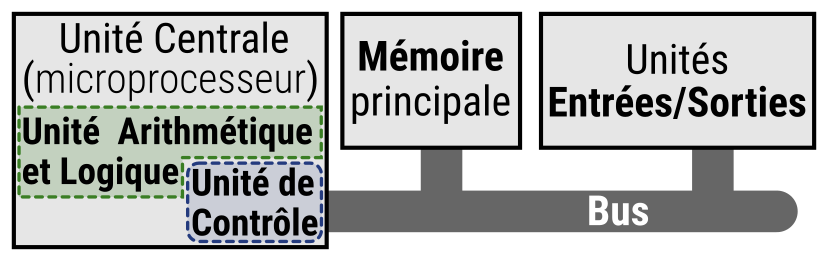
\includegraphics{./res/archi.png}

Cerveau de la machine, l'unité centrale (ou \emph{microprocesseur}) est
constituée d'une \textbf{unité arithmétique et logique} (pour effectuer
les calculs) et d'une \textbf{unité de contrôle} (pour pilote les
échanges à travers le \textbf{Bus}.

La \textbf{mémoire} contient à la fois les données et les programmes.

Les périphériques d'\textbf{entrées/sorties} permettent d'envoyer ou de
recevoir des données avec l'extérieur (clavier, souris, écran,
imprimante, etc.).

        \end{retenir}
    \hypertarget{premier-programme-avec-la-carte-textttmicrobit}{%
\subsubsection{\texorpdfstring{4.1.2 --- Premier programme avec la carte
\(\texttt{Micro:bit}\)}{4.1.2 --- Premier programme avec la carte \textbackslash texttt\{Micro:bit\}}}\label{premier-programme-avec-la-carte-textttmicrobit}}
\begin{eleve}
    \textbf{D'après toi}, que fait le programme ci-dessous ?

\begin{Shaded}
\begin{Highlighting}[]
\ImportTok{from}\NormalTok{ microbit }\ImportTok{import} \OperatorTok{*}
\NormalTok{e0 }\OperatorTok{=}\NormalTok{ button\_a.is\_pressed()}
\ControlFlowTok{if}\NormalTok{ e0:}
\NormalTok{    display.show(}\StringTok{"1"}\NormalTok{)}
\ControlFlowTok{else}\NormalTok{:}
\NormalTok{    display.show(}\StringTok{"0"}\NormalTok{)}
\end{Highlighting}
\end{Shaded}

\textbf{Ouvrir} l'éditeur \texttt{Mu-editor}, \textbf{recopier} ce
programme et le \textbf{téléverser} sur la carte (bouton
\texttt{Flasher} 
\includegraphics{res/flash.png}).

\begin{enumerate}
\def\labelenumi{\arabic{enumi}.}
\setcounter{enumi}{1}
\tightlist
\item
  \textbf{Observe} le fonctionnement de la carte et \textbf{propose} une
  ou plusieurs interprétations (pour confirmer/infirmer tes
  observations, tu peux manipuler les boutons présents sur la carte : A
  / B / Reset).
\end{enumerate}

\textbf{Présenter} tes réponses au professeur.

\begin{enumerate}
\def\labelenumi{\arabic{enumi}.}
\setcounter{enumi}{2}
\tightlist
\item
  \textbf{Indique} le nombre de fois qu'est exécutée l'instruction
  conditionnelle.
\item
  \textbf{D'après toi}, combien de fois doit être exécutée l'instruction
  conditionnelle pour que la carte reste à l'écoute des entrées et
  réagisse chaque fois que l'état du bouton A change ?
\item
  \textbf{Améliore} le programme en tenant compte de tes observations et
  de tes réponses aux questions précédentes.
\end{enumerate}

\textbf{Présente} la carte programmée au professeur.

La fonction \texttt{button\_a.is\_pressed()} peut être avantageusement
remplacée par un appel à la fonction \texttt{button\_a.was\_pressed()}.

Son appel renvoie une valeur booléenne \texttt{True} (vrai) ou
\texttt{False} (faux) et permet de savoir si le bouton A \emph{a été
pressé} depuis la dernière fois que cette fonction a été appelée. Cette
fonction renvoie \texttt{True} s'il a été pressé entre deux appels et
\texttt{False} sinon.

\begin{enumerate}
\def\labelenumi{\arabic{enumi}.}
\setcounter{enumi}{5}
\tightlist
\item
  \textbf{Modifie} le programme pour que l'affichage \texttt{0/1} change
  uniquement lorsque l'on presse le bouton A (et pas lorsqu'on le
  relâche).
\end{enumerate}
        
        \end{eleve}
    \hypertarget{commandes-de-base-pour-programmer-avec-textttmicrobit}{%
\subsection{\texorpdfstring{4.2 --- Commandes de base pour programmer
avec
\(\texttt{Micro:bit}\)}{4.2 --- Commandes de base pour programmer avec \textbackslash texttt\{Micro:bit\}}}\label{commandes-de-base-pour-programmer-avec-textttmicrobit}}

    Dans la suite, tu utiliseras l'éditeur \texttt{mu-editor} pour
programmer ta carte \(\texttt{Micro:bit}\). Si tu le souhaites tu
pourras, \textbf{sur ton temps personnel}, essayer de programmer la
carte avec VSCodium\ldots{}

    3.2.1 --- La bibliothèque \texttt{microbit}

    En Python, les entrées/sorties de la carte \(\texttt{Micro:bit}\) ne
sont pas \emph{nativement} accessibles. Afin de pouvoir utiliser les
fonctions prévues à cet effet, il faut utiliser la bibliothèque
\texttt{microbit}.
\begin{exemple}
    Pour importer cette bibliothèque, il faut utiliser la commande:

\begin{Shaded}
\begin{Highlighting}[]
\ImportTok{from}\NormalTok{ microbit }\ImportTok{import} \OperatorTok{*}
\end{Highlighting}
\end{Shaded}

        \end{exemple}
    L'utilisation de cette bibliothèque nous permettra d'utiliser
différentes fonctionnalités de la carte \(\texttt{Micro:bit}\) :

\begin{itemize}
\tightlist
\item
  \textbf{Image} pour créer et manipuler les images.
\item
  \textbf{Button} avec deux \emph{instances} \texttt{button\_a} et
  \texttt{button\_b} pour connaître l'état des boutons.
\item
  \textbf{Pin} avec différentes \emph{instances} en fonction du type de
  broche (par exemple \texttt{pin0}, \texttt{pin1} et \texttt{pin2}).
\item
  \textbf{display} pour gérer l'écran de LED
\item
  \textbf{accelerometer} pour interroger l'accéléromètre
\item
  \textbf{compass} pour manipuler et interroger la boussole
\item
  \textbf{music} pour créer et manipuler de la musique
\item
  \textbf{speech} pour faire parler le \(\texttt{Micro:bit}\)
\item
  \textbf{radio} pour communiquer entres plusieurs
  \(\texttt{Micro:bit}\) via un protocole simple.
\end{itemize}

    \hypertarget{micropython-dans-la-carte-textttmicrobit}{%
\subsubsection{\texorpdfstring{4.2.2 --- Micropython dans la carte
\(\texttt{Micro:bit}\)}{4.2.2 --- Micropython dans la carte \textbackslash texttt\{Micro:bit\}}}\label{micropython-dans-la-carte-textttmicrobit}}

    Lorsque la carte \(\texttt{Micro:bit}\) est flashée par
\texttt{mu-editor} avec la bibliothèque \texttt{microbit}, elle contient
un noyau \emph{micropython}. Il est alors possible d'écrire du code qui
sera interprété par ce noyau micropython de la carte.

Pour accéder à l'interprète Python de la carte, il suffit de cliquer sur
l'icône REPL de l'application.
\begin{exemple}
    Pour utiliser le terminal de la carte \(\texttt{Micro:bit}\) :

\begin{enumerate}
\def\labelenumi{\arabic{enumi}.}
\tightlist
\item
  Flasher la carte \(\texttt{Micro:bit}\) avec micropython.
\item
  Ouvrir le terminal de la carte en cliquant sur REPL
\item
  Écrire le code ci-dessous :
\end{enumerate}

\begin{Shaded}
\begin{Highlighting}[]
\BuiltInTok{print}\NormalTok{(}\StringTok{"Hello, World!"}\NormalTok{)}
\end{Highlighting}
\end{Shaded}

        \end{exemple}
    \hypertarget{afficher-un-texte}{%
\subsubsection{4.2.3 --- Afficher un texte}\label{afficher-un-texte}}

    Le module \texttt{display} permet de gérer l'écran de LED de
\(\texttt{Micro:bit}\). Les fonctionnalités offertes par ce module sont
accessible en ajoutant un point
\texttt{\textquotesingle{}.\textquotesingle{}} après
\texttt{\textquotesingle{}display\textquotesingle{}} puis en écrivant le
nom de la fonction à appeler :

\begin{itemize}
\tightlist
\item
  \texttt{display.show(mon\_texte)} permet d'afficher la chaîne de
  caractère contenue dans la variable \texttt{mon\_texte}
\item
  \texttt{display.scroll(mon\_texte)} permet de la
  \(\texttt{Micro:bit}\)
\item
  \texttt{display.clear()} permet d'effacer l'écran.
\end{itemize}
\begin{eleve}
    \(\texttt{Micro:bit}\) le mot \texttt{Hello} puis afficher la chaîne
\texttt{World!}.
        
        \end{eleve}\begin{reponse}
        {\scriptsize
    \begin{tcolorbox}[breakable, size=fbox, boxrule=1pt, pad at break*=1mm,colback=cellbackground, colframe=cellborder]
\prompt{In}{incolor}{ }{\boxspacing}
\begin{Verbatim}[commandchars=\\\{\}]
\PY{k+kn}{from} \PY{n+nn}{microbit} \PY{k+kn}{import} \PY{o}{*}
\PY{n}{display}\PY{o}{.}\PY{n}{scroll}\PY{p}{(}\PY{l+s+s2}{\PYZdq{}}\PY{l+s+s2}{Hello,}\PY{l+s+s2}{\PYZdq{}}\PY{p}{)}
\PY{n}{display}\PY{o}{.}\PY{n}{show}\PY{p}{(}\PY{l+s+s2}{\PYZdq{}}\PY{l+s+s2}{World!}\PY{l+s+s2}{\PYZdq{}}\PY{p}{)}
\end{Verbatim}
\end{tcolorbox}
    }

        \end{reponse}
    \hypertarget{des-images}{%
\subsubsection{4.2.4 --- Des images}\label{des-images}}

    La classe \texttt{Image} contient comme \emph{attributs} de nombreuses
images pré-programmées. Ces constantes sont accessibles grâce à un point
\texttt{\textquotesingle{}.\textquotesingle{}} placé après
\texttt{\textquotesingle{}Image\textquotesingle{}}. Par exemple l'image
du coeur est accessible via l'instruction \texttt{Image.HEART} :

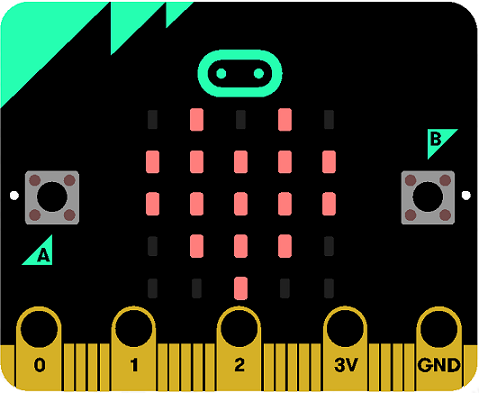
\includegraphics{res/mbpy-init-heart.png}

Comme pour les textes, les images s'affichent grâce à l'instruction
\texttt{display.show()}.
\begin{exemple}
    Voici par exemple comment afficher successivement des images : une image
est affichée pendant une seconde puis ensuite une autre image s'affiche.
Une seconde plus tard, l'écran s'efface.

\begin{Shaded}
\begin{Highlighting}[]
\ImportTok{from}\NormalTok{ microbit }\ImportTok{import} \OperatorTok{*}
\NormalTok{display.show(Image.HAPPY)}
\NormalTok{sleep(}\DecValTok{1000}\NormalTok{)}
\NormalTok{display.show(Image.ANGRY)}
\NormalTok{sleep(}\DecValTok{1000}\NormalTok{)}
\NormalTok{display.clear()}
\end{Highlighting}
\end{Shaded}

Il faut mettre le \(\texttt{Micro:bit}\) en pause. Sinon l'utilisateur
n'aura pas le temps de tout voir. La commande \texttt{sleep(duree)}
arrête donc la carte pendant une durée \texttt{duree} exprimée en
milliseconde par un nombre entier (int).

        \end{exemple}
    \hypertarget{des-boutons}{%
\subsubsection{4.2.5 --- Des boutons}\label{des-boutons}}

    Pour connaître les états des boutons de la carte \(\texttt{Micro:bit}\)
on utilise les classes \texttt{button\_a} (pour le bouton A de la carte)
et \texttt{button\_b} (pour le bouton B).

Comme d'habitude, les fonctionnalités offertes par ces classes sont
accessibles via un point \texttt{\textquotesingle{}.\textquotesingle{}}
placé après le nom de la classe :

\begin{itemize}
\tightlist
\item
  \texttt{.get\_presses()} renvoie le \textbf{nombre} de fois que le
  bouton a été pressé depuis le dernier appel de cette fonction
\item
  \texttt{.is\_pressed()} renvoie une \textbf{valeur booléenne} (vrai
  \texttt{True} ou fausse \texttt{False}) qui indique si le bouton est
  \emph{actuellement} pressé
\item
  \texttt{.was\_pressed()} renvoie une \textbf{valeur booléenne} qui
  indique si le bouton \emph{a été} pressé depuis le dernier appel de
  cette méthode.
\end{itemize}
\begin{eleve}
    Écris un code permettant d'afficher le nombre de fois que le bouton B a
été pressé dans les 10 secondes qui ont suivies l'alimentation de la
carte.

\emph{(bon à savoir) : la fonction \texttt{str(nb)} permet de
transformer le nombre en entier \texttt{nb} en une chaîne de caractère
qu'on peut \(\texttt{Micro:bit}\).}
        
        \end{eleve}\begin{reponse}
        {\scriptsize
    \begin{tcolorbox}[breakable, size=fbox, boxrule=1pt, pad at break*=1mm,colback=cellbackground, colframe=cellborder]
\prompt{In}{incolor}{ }{\boxspacing}
\begin{Verbatim}[commandchars=\\\{\}]
\PY{k+kn}{from} \PY{n+nn}{microbit} \PY{k+kn}{import} \PY{o}{*}
\PY{n}{sleep}\PY{p}{(}\PY{l+m+mi}{10000}\PY{p}{)}
\PY{n}{display}\PY{o}{.}\PY{n}{scroll}\PY{p}{(}\PY{n+nb}{str}\PY{p}{(} \PY{n}{button\PYZus{}a}\PY{o}{.}\PY{n}{get\PYZus{}presses}\PY{p}{(}\PY{p}{)} \PY{p}{)}\PY{p}{)}
\end{Verbatim}
\end{tcolorbox}
    }

        \end{reponse}
    Une carte \(\texttt{Micro:bit}\) est un objet connecté qui, entres
autres, est à l'écoute de certains \textbf{évènements}. Pour programmer
cette capacité d'écoute, il est possible d'appliquer le principe
fondamental des objets connectés : créer une \textbf{boucle infinie}
\texttt{while\ True:}.

À chaque tour de cette boucle, le programme doit vérifier la réalisation
de l'évènement attendu.

Lorsque l'événement se réalise, il est possible d'utiliser le mot clé
\texttt{break} qui permet alors de quitter la boucle infinie.
\begin{exemple}
    Le programme ci-dessous tourne en boucle :

\begin{itemize}
\tightlist
\item
  Lorsque aucun évènement n'est détecté, c'est l'image triste
  \texttt{Image.SAD} qui s'affiche.
\item
  Pendant que le bouton A est pressé, l'image joyeuse
  \texttt{Image.HAPPY} s'affiche.
\item
  Pendant que la broche \texttt{pin1} est touchée (pour cela, pincer en
  même temps que la broche \texttt{GND} avec la main droite et la broche
  \texttt{pin1} avec la main gauche), l'image endormie
  \texttt{Image.ASLEEP} s'affiche.
\item
  Enfin, lorsque le bouton B est pressé, l'écran s'efface et le
  programme quitte la boucle.
\end{itemize}

\begin{Shaded}
\begin{Highlighting}[]
\ImportTok{from}\NormalTok{ microbit }\ImportTok{import} \OperatorTok{*}
\ControlFlowTok{while} \VariableTok{True}\NormalTok{:}
    \ControlFlowTok{if}\NormalTok{ button\_a.is\_pressed():}
\NormalTok{        display.show(Image.HAPPY)}
    \ControlFlowTok{elif}\NormalTok{ pin1.is\_touched():}
\NormalTok{        display.show(Image.ASLEEP)}
    \ControlFlowTok{elif}\NormalTok{ button\_b.is\_pressed():}
\NormalTok{        display.clear()}
        \ControlFlowTok{break}
    \ControlFlowTok{else}\NormalTok{:}
\NormalTok{        display.show(Image.SAD)}
\end{Highlighting}
\end{Shaded}

        \end{exemple}\begin{remarque}
    Les broches \texttt{pin0}, \texttt{pin1} et \texttt{pin2} peuvent aussi
servir de bouton. Ainsi la méthode \texttt{.is\_touched()}\} permet de
renvoyer une valeur booléenne qui vaut \texttt{True} lorsqu'une personne
en contact avec la masse (broche \texttt{GND}) touche puis relâche la
broche en question.

En effet quand l'instruction est exécutée, la carte mesure la résistance
entre la broche à laquelle l'instruction s'applique et la masse (broche
\texttt{GND}). Si cette dernière a varié et est passée d'une valeur
quasi infinie à une valeur faible, le test devient vrai (\texttt{True}).
Cet évènement arrive lorsqu'une personne en contact avec \texttt{GND}
touche la broche puis la relâche.

        \end{remarque}
    \hypertarget{le-hasard}{%
\subsubsection{4.2.6 Le hasard}\label{le-hasard}}

La bibliothèque \texttt{random} est utilisable avec
\(\texttt{Micro:bit}\). Grâce à cette bibliothèque, il est très simple
de générer des nombres aléatoires avec les fonctions :

\begin{itemize}
\tightlist
\item
  \texttt{random()} pour tirer un nombre décimal (\texttt{float})
  compris entre 0 (inclus) et 1 (exclu)
\item
  \texttt{randint(a,b)} pour tirer un nombre entier (\texttt{int})
  appartenant à \texttt{a..b} (inclus).
\end{itemize}
\begin{exemple}
    Le programme ci-dessous affiche très rapidement 50 nombres aléatoires
tirés entre 1 et 6. Le dernier nombre tiré est affiché pendant une
seconde puis effacé.

\begin{Shaded}
\begin{Highlighting}[]
\ImportTok{from}\NormalTok{ microbit }\ImportTok{import} \OperatorTok{*}
\ImportTok{from}\NormalTok{ random }\ImportTok{import}\NormalTok{ randint}
\ControlFlowTok{for}\NormalTok{ i }\KeywordTok{in} \BuiltInTok{range}\NormalTok{(}\DecValTok{50}\NormalTok{):}
\NormalTok{    display.show(random.randint(}\DecValTok{1}\NormalTok{, }\DecValTok{6}\NormalTok{))}
\NormalTok{    sleep(}\DecValTok{20}\NormalTok{)}
\NormalTok{sleep(}\DecValTok{1000}\NormalTok{)}
\NormalTok{display.clear()}
\end{Highlighting}
\end{Shaded}

        \end{exemple}
    \hypertarget{le-mouvement}{%
\subsubsection{4.2.7 --- Le mouvement}\label{le-mouvement}}

L'accéléromètre de la carte \(\texttt{Micro:bit}\) est accessible par le
module \texttt{accelerometer}.

Il est alors possible de récupérer une des coordonnées du vecteur
accélération. Par exemple avec un appel à la fonction
\texttt{.get\_x()}.
\begin{exemple}
    Le programme ci-dessous affiche une flèche en fonction de l'inclinaison
de la carte \(\texttt{Micro:bit}\).

Le bouton B permet de quitter la boucle infinie.

\begin{Shaded}
\begin{Highlighting}[]
\ImportTok{from}\NormalTok{ microbit }\ImportTok{import} \OperatorTok{*}
\NormalTok{button\_b.was\_pressed()}
\ControlFlowTok{while} \VariableTok{True}\NormalTok{:}
\NormalTok{    capteur }\OperatorTok{=}\NormalTok{ accelerometer.get\_x()}
    \ControlFlowTok{if}\NormalTok{ capteur }\OperatorTok{\textgreater{}} \DecValTok{40}\NormalTok{:}
\NormalTok{        display.show(Image.ARROW\_E)}
    \ControlFlowTok{elif}\NormalTok{ capteur }\OperatorTok{\textless{}} \OperatorTok{{-}}\DecValTok{40}\NormalTok{:}
\NormalTok{        display.show(Image.ARROW\_W)}
    \ControlFlowTok{else}\NormalTok{:}
\NormalTok{        display.show(}\StringTok{"{-}"}\NormalTok{)}
        
    \ControlFlowTok{if}\NormalTok{ button\_b.was\_pressed():}
\NormalTok{        display.clear()}
        \ControlFlowTok{break}
\end{Highlighting}
\end{Shaded}

        \end{exemple}
    \hypertarget{les-gestes}{%
\subsubsection{4.2.8 --- Les gestes}\label{les-gestes}}

Le module \texttt{accelerometer} peut aussi détecter des mouvements ou
des positions pré-programmés : les \emph{gestes}
(\texttt{\textquotesingle{}up\textquotesingle{}},
\texttt{\textquotesingle{}down\textquotesingle{}},
\texttt{\textquotesingle{}left\textquotesingle{}},
\texttt{\textquotesingle{}right\textquotesingle{}},
\texttt{\textquotesingle{}face\ up\textquotesingle{}},
\texttt{\textquotesingle{}face\ down\textquotesingle{}},
\texttt{\textquotesingle{}freefall\textquotesingle{}},
\texttt{\textquotesingle{}3g\textquotesingle{}},
\texttt{\textquotesingle{}6g\textquotesingle{}},
\texttt{\textquotesingle{}8g\textquotesingle{}},
\texttt{\textquotesingle{}shake\textquotesingle{}}).
\begin{remarque}
    L'utilisation des gestes est très lente.

        \end{remarque}
    Pour cela, il existe :

\begin{itemize}
\tightlist
\item
  \texttt{accelerometer.get\_gestures()} qui renvoie un ensemble appelé
  \texttt{tuple} contenant l'historique des gestes. Le dernier élément
  du tuple est le geste le plus récent. Le tuple est réinitialisé à
  chaque appel de cette fonction.
\item
  \texttt{accelerometer.is\_gesture(nom\_du\_geste)} qui renvoie une
  \textbf{valeur booléenne} indiquant si le geste en cours est
  \texttt{nom\_du\_geste}
\item
  \texttt{accelerometer.was\_pressed(nom\_du\_geste)} qui renvoie une
  \textbf{valeur booléenne} indiquant si le geste
  \texttt{nom\_du\_geste} \emph{a été} pressé depuis le dernier appel de
  cette fonction.
\end{itemize}
\begin{exemple}
    Le programme ci-dessous affiche le nombre ``8''.

Lorsque la carte \(\texttt{Micro:bit}\) est secoué, il s'affiche une
seconde plus tard de manière aléatoire et équiprobable soit
\texttt{"Oui"}, soit \texttt{"Non"}.

Après une petite pause, le jeu recommence sauf si on appui sur le bouton
B ce qui fait sortir de la boucle.

\begin{Shaded}
\begin{Highlighting}[]
\ImportTok{from}\NormalTok{ microbit }\ImportTok{import} \OperatorTok{*}
\ImportTok{from}\NormalTok{ random }\ImportTok{import}\NormalTok{ choice}
\NormalTok{button\_b.was\_pressed()}
\ControlFlowTok{while} \VariableTok{True}\NormalTok{:}
\NormalTok{    display.show(}\StringTok{"8"}\NormalTok{)}
    \ControlFlowTok{if}\NormalTok{ accelerometer.was\_gesture(}\StringTok{"shake"}\NormalTok{):}
\NormalTok{        display.clear()}
\NormalTok{        sleep(}\DecValTok{1000}\NormalTok{)}
\NormalTok{        display.scroll(random.choice([}\StringTok{"Oui"}\NormalTok{,}\StringTok{"Non"}\NormalTok{]))}
\NormalTok{        sleep(}\DecValTok{250}\NormalTok{)}
    \ControlFlowTok{if}\NormalTok{ button\_b.was\_pressed():}
        \ControlFlowTok{break}
\end{Highlighting}
\end{Shaded}

        \end{exemple}
    \hypertarget{la-radio}{%
\subsubsection{4.2.9 --- La radio}\label{la-radio}}

Les cartes \(\texttt{Micro:bit}\) peuvent communiquer entres elles au
moyen du module \texttt{radio}.

\begin{itemize}
\tightlist
\item
  \texttt{radio.send(texte)} permet d'envoyer par radio la chaîne de
  caractère \texttt{texte}.
\item
  \texttt{radio.receive()} renvoie les données reçues par radio
  converties en une chaîne de caractère. Si rien n'a été reçu, la chaîne
  vaut \texttt{None}.
\end{itemize}
\begin{exemple}
    Le programme ci dessous est à téléverser sur 2 cartes
\(\texttt{Micro:bit}\). Il contient à la fois une partie émetteur et une
partie récepteur. Un appui sur les boutons A ou B de l'une ou l'autre
des cartes \(\texttt{Micro:bit}\) affiche les texte ``A'' ou ``B'' sur
l'autre. Un appui sur la broche \texttt{pin0} arrête le programme.

\begin{Shaded}
\begin{Highlighting}[]
\ImportTok{from}\NormalTok{ microbit }\ImportTok{import} \OperatorTok{*}
\NormalTok{button\_a.was\_pressed()}
\NormalTok{button\_b.was\_pressed()}
\ControlFlowTok{while} \VariableTok{True}\NormalTok{:}
    \CommentTok{\# émetteur}
    \ControlFlowTok{if}\NormalTok{ button\_a.was\_pressed():}
\NormalTok{        radio.send(}\StringTok{"A"}\NormalTok{)}
    \ControlFlowTok{if}\NormalTok{ button\_b.was\_pressed():}
\NormalTok{        radio.send(}\StringTok{"B"}\NormalTok{)}
    \CommentTok{\# récepteur}
\NormalTok{    message }\OperatorTok{=}\NormalTok{ radio.receive()}
    \ControlFlowTok{if}\NormalTok{ message }\OperatorTok{==} \StringTok{"A"}\NormalTok{:}
\NormalTok{        display.scroll(}\StringTok{"A"}\NormalTok{)}
    \ControlFlowTok{if}\NormalTok{ message }\OperatorTok{==} \StringTok{"B"}\NormalTok{:}
\NormalTok{        display.scroll(}\StringTok{"B"}\NormalTok{)}
    \CommentTok{\# pause pour éviter de saturer la carte}
\NormalTok{    sleep(}\DecValTok{20}\NormalTok{)}
    \CommentTok{\# sortir de la boucle}
    \ControlFlowTok{if}\NormalTok{ pin0.is\_touched():}
\NormalTok{        display.clear()}
        \ControlFlowTok{break}
\end{Highlighting}
\end{Shaded}

        \end{exemple}
    \hypertarget{la-boussole}{%
\subsubsection{4.2.10 --- La boussole}\label{la-boussole}}

Pour utiliser la boussole de la carte \(\texttt{Micro:bit}\), il faut
utiliser le module \texttt{compass}.

\begin{itemize}
\tightlist
\item
  \texttt{compass.get\_x()} (ou \texttt{.get\_y()} ou
  \texttt{.get\_y()}) renvoient une des composantes du vecteur champ
  magnétique.
\item
  \texttt{compass.heading()} renvoie un nombre entier (\texttt{int})
  correspondant à l'angle en degré entre l'orientation de la carte
  \(\texttt{Micro:bit}\) et le nord magnétique.
\end{itemize}
\begin{remarque}
    Avant d'utiliser une fonctionnalité du module \texttt{compass}, il faut
obligatoirement \emph{calibrer} la carte. Sans cela, les valeurs
renvoyées sont fausses à cause du \emph{bruit magnétique} présent dans
l'environnement de la carte.

Au moment de calibrer la boussole, l'utilisateur doit bouger la carte
dans différentes positions jusqu'à faire passer le point clignotant par
toutes les LED de l'écran.

L'outil de calibration se lance automatiquement mais il est possible de
programmer son exécution en appelant l'instruction
\texttt{compass.calibrate()}.

        \end{remarque}\begin{exemple}
    Le programme ci-dessous fait office de boussole et indique le nord
magnétique.

Attention, le capteur est sensible aux objets tels que téléphones,
ordinateurs ou aux lieux tels que ascenseurs ou salle
informatique\ldots{}

\begin{Shaded}
\begin{Highlighting}[]
\ImportTok{from}\NormalTok{ microbit }\ImportTok{import} \OperatorTok{*}
\NormalTok{compass.calibrate()}
\NormalTok{button\_b.was\_pressed()}
\ControlFlowTok{while} \VariableTok{True}\NormalTok{:}
\NormalTok{    cap }\OperatorTok{=}\NormalTok{ ((}\DecValTok{15} \OperatorTok{{-}}\NormalTok{ compass.heading()) }\OperatorTok{//} \DecValTok{30}\NormalTok{) }\OperatorTok{\%} \DecValTok{12}
\NormalTok{    display.show(Image.ALL\_CLOCKS[cap])}
    \ControlFlowTok{if}\NormalTok{ button\_b.was\_pressed():}
\NormalTok{        display.clear()}
        \ControlFlowTok{break}
\end{Highlighting}
\end{Shaded}

        \end{exemple}
    \hypertarget{nuages-de-points-avec-mu-editor}{%
\subsubsection{\texorpdfstring{4.2.11 --- Nuages de points avec
\texttt{Mu-editor}}{4.2.11 --- Nuages de points avec Mu-editor}}\label{nuages-de-points-avec-mu-editor}}

Il est possible de tracer un \textbf{nuage de points} avec l'éditeur
\texttt{Mu-editor}.

Pour cela, il faut

\begin{itemize}
\tightlist
\item
  utiliser l'outil \texttt{Graphique} de \texttt{Mu-editor},
\item
  faire afficher par le programme en cours d'exécution un \texttt{tuple}
  de nombres.
\end{itemize}
\begin{exemple}
    Le programme ci-dessous affiche dans le terminal (ou dans le
\textbf{Graphique} si l'outil de l'IDE est cliqué) deux nombres
aléatoires appartenant à -100..100.

\begin{Shaded}
\begin{Highlighting}[]
\ImportTok{from}\NormalTok{ microbit }\ImportTok{import} \OperatorTok{*}
\ImportTok{from}\NormalTok{ random }\ImportTok{import}\NormalTok{ randint}
\NormalTok{drapeau }\OperatorTok{=} \VariableTok{True}
\ControlFlowTok{while} \VariableTok{True}\NormalTok{:}
\NormalTok{    sleep(}\DecValTok{50}\NormalTok{)}
    \ControlFlowTok{if}\NormalTok{ button\_a.was\_pressed():}
\NormalTok{        drapeau }\OperatorTok{=} \KeywordTok{not}\NormalTok{ drapeau}
    \ControlFlowTok{if}\NormalTok{ drapeau:}
\NormalTok{        nb1 }\OperatorTok{=}\NormalTok{ randint(}\OperatorTok{{-}}\DecValTok{100}\NormalTok{,}\DecValTok{100}\NormalTok{)}
\NormalTok{        nb2 }\OperatorTok{=}\NormalTok{ randint(}\OperatorTok{{-}}\DecValTok{100}\NormalTok{,}\DecValTok{100}\NormalTok{)}
        \BuiltInTok{print}\NormalTok{( (nb1,nb2) )}
\end{Highlighting}
\end{Shaded}

        \end{exemple}

    % Add a bibliography block to the postdoc
    
    
    
\end{document}
